\setcounter{ExampleCounter}{1}
We began by calculating the probabilities of single events occurring, and then we learned how to combine events using \emph{OR}.  Now we ask a different question: suppose we know how to calculate the probability of $A$ and the probability of $B$ on their own; how can we calculate the probability that $A$ \emph{AND} $B$ both occur?  To set this up, we'll look at two situations: flipping a coin twice and drawing two cards \emph{without replacement} (this will be important).

\paragraph{Flipping a coin twice} If\marginnote{Independent events:\\ don't affect each other\\ (whether the first flip is heads or tails, the probabilities for the second flip are not impacted)} we flip a coin twice in succession, the sample space is \[S=\{HH, HT, TH, TT\}.\]  Now suppose we ask the following questions:
\begin{enumerate}
\item What is the probability that the first flip results in a head?
\begin{center}
Either by noticing that there are two possibilities for the first flip or by looking at the sample space and seeing that there are two outcomes (out of four total) that correspond to a head on the first flip, we can reason that this probability is 1/2.
\end{center} 
\item What is the probability that the second flip results in a tail?
\begin{center}
Using the same reasoning, we conclude that this probability is also 1/2.
\end{center} 
\item What is the probability that the first flip results in a head \emph{AND} the second flip results in a tail?
\begin{center}
Looking at the sample space, we notice that there is exactly one outcome that corresponds to this (out of four), so this probability is 1/4.
\end{center}
\end{enumerate}

Notice that the probability of both happening together is the probability of one times the probability of the other:
\[\dfrac{1}{2} \cdot \dfrac{1}{2} = \dfrac{1}{4}\]

Seeing this, and noting the title of the section, we may be tempted to jump to the conclusion that the probability of $A$ \emph{AND} $B$ is simply the probability of $A$ times the probability of $B$.  However, the next scenario illustrates that we need to be a bit more careful.

Just as we found with the addition rule, there is a simple version that works if a certain condition is met, and if not, there is a more general version of the multiplication rule.

\paragraph{Drawing two cards without replacement}
Suppose\marginnote{Dependent events:\\ affect each other\\ (after pulling out the first card, the deck has changed, so the probabilities have shifted)} we draw one card, and then \emph{without} placing it back and re-shuffling the deck, we draw a second card.  What is the probability that we draw two Aces?\\

This situation is different from the previous one, because now what happens on the first draw affects the probabilities for the second draw.  In other words, the probability of drawing an Ace the first time is 4/52.  If we draw an Ace the first time, there are only 3 Aces left and 51 total cards left, so the probability of drawing an Ace the second time is 3/51.  However, if we do not draw an Ace the first time, there are still 4 Aces in the deck, so the probability of drawing an Ace the second time is 4/51.  We can illustrate this with a branching tree diagram.

\begin{center}
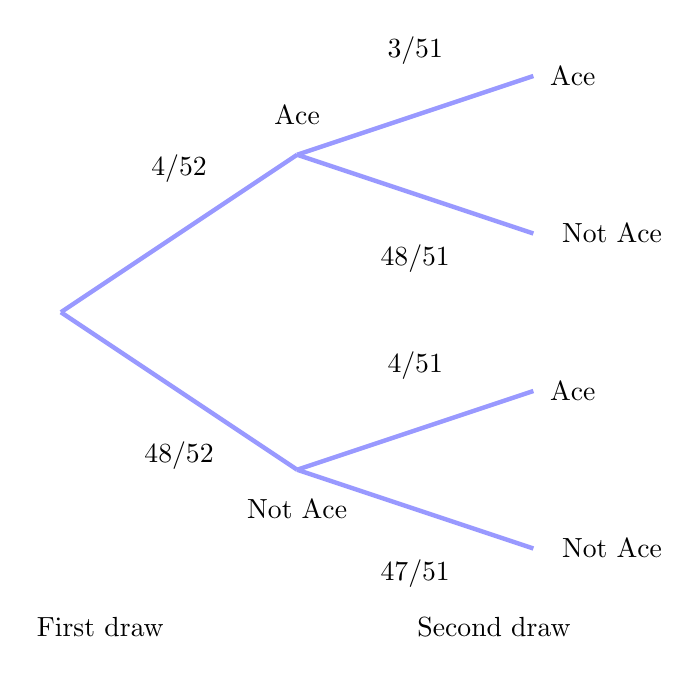
\begin{tikzpicture}
\draw [ultra thick,color=blue!40] (-3,0) -- (0,2) node[midway, above, yshift=0.5cm, color=black] {4/52};
\draw [ultra thick,color=blue!40] (0,2) -- (3,3) node[midway, above, yshift=0.5cm, color=black] {3/51};
\draw [ultra thick,color=blue!40] (0,2) -- (3,1) node[midway, below, yshift=-0.5cm, color=black] {48/51};

\draw [ultra thick,color=blue!40] (-3,0) -- (0,-2) node[midway, below, yshift=-0.5cm, color=black] {48/52};
\draw [ultra thick,color=blue!40] (0,-2) -- (3,-1) node[midway, above, yshift=0.5cm, color=black] {4/51};
\draw [ultra thick,color=blue!40] (0,-2) -- (3,-3) node[midway, below, yshift=-0.5cm, color=black] {47/51};

\draw [yshift=-4cm,xshift=-2.5cm] node {First draw};
\draw [yshift=-4cm,xshift=2.5cm] node {Second draw};
\draw [yshift=2.5cm,xshift=0cm] node {Ace};
\draw [yshift=-2.5cm,xshift=0cm] node {Not Ace};
\draw [yshift=3cm,xshift=3.5cm] node {Ace};
\draw [yshift=1cm,xshift=4cm] node {Not Ace};
\draw [yshift=-1cm,xshift=3.5cm] node {Ace};
\draw [yshift=-3cm,xshift=4cm] node {Not Ace};

\end{tikzpicture}
\end{center}

Now the probability of drawing an Ace both times is the probability of drawing an Ace the first time multiplied by the probability of drawing an Ace the second time \textbf{given that we drew an Ace the first time}.  Notice on the tree diagram that this corresponds to following the upward branch both times.

This is because \emph{only} if we draw an Ace the first time do we have any chance of fulfilling the scenario; if we fail to draw an Ace the first time, it doesn't matter what we do the second time--we've already failed.

Thus, the probability of drawing an Ace both times is 
\begin{center}
$P($Ace the first time$) \cdot P($Ace the second time IF we drew one the first time$)$\\
\text{}\\
$= \dfrac{4}{52} \cdot \dfrac{3}{51} = \dfrac{12}{2652} \approx 0.0045$
\end{center}

This is what we call \emph{conditional probability}, and it's what we have to consider for the general multiplication rule.

\subsection{Independence}
What was the difference between those two scenarios?  Why, in the first one, could we simply multiply the individual probabilities and in the second we had to think about conditional probability?  The answer lies in what we call \textbf{independence}: when flipping the coin, each time we flipped it had no impact on the other times; when we drew the cards without replacement, though, one draw affected the next.  Notice that we made the careful distinction that we drew without replacement; if we had replaced the first card and re-shuffled the deck before drawing again, the two draws would have been independent.

\begin{proc}{Independence}
Two events are independent if the outcome of one has no effect on the probability of the other occurring.
\end{proc}

Note that saying that two events are \emph{independent} is different than saying that two events are \emph{mutually exclusive}.
\begin{itemize}
\item If two events are independent, they have no effect on each other's likelihood of occurring.
\item If two events are mutually exclusive, they cannot occur together, so they do have an effect on each other's likelihood of occurring (namely, making it impossible).
\end{itemize}
\pagebreak

\begin{example}[https://www.youtube.com/watch?v=ul4iYkGHbAE]{Independent events}
Determine whether these events are independent:

\begin{enumerate}
\item A fair coin is tossed two times. The two events are $A$ =  first toss is Heads and $B$ =  second toss is Heads.
\begin{center}
The\marginnote{\bfseries Solution} probability that Heads comes up on the second toss is 1/2 regardless of whether or not Heads came up on the first toss, so these events are independent.
\end{center}

\item The two events $A$ =  \emph{It will rain tomorrow in Frederick MD} and $B$ =  \emph{It will rain tomorrow in Thurmont MD} 
\begin{center}
These\marginnote{\bfseries Solution} events are not independent because it is more likely that it will rain in Thurmont on days it rains in Frederick.
\end{center} 

\item You draw a red card from a deck, then draw a second card without replacing the first.
\begin{center}
These\marginnote{\bfseries Solution} events are dependent, specifically because the first card is \textit{not replaced}.  After drawing the first card, the deck looks different than it did before.  There are 25 red cards left and 26 black cards left, so the probabilities have shifted.
\end{center}

\item You draw a face card from the deck, then replace it and re-shuffle the deck before drawing a second card.
\begin{center}
Since\marginnote{\bfseries Solution} you reset the deck between draws, the events are independent.
\end{center}
\end{enumerate}
\end{example}

Now we are ready to formally state the rule that we used in the first scenario at the beginning of the section.
\vspace*{-0.1in}

\subsection{The Multiplication Rule for Independent Events}
\begin{formula}{Probabilities of independent events}
If $A$ and $B$ are independent, then the probability of both $A$ and $B$ occurring is
\[  P( A \mbox{ and } B) = P(A) \cdot P(B) \]

We can generalize this to finitely many independent events $A_1, A_2, \dots, A_k$
\[ P( A_1 \mbox{ and } A_2 \mbox{ and } \dots \mbox{ and } A_k ) = P(A_1) \cdot P(A_2) \cdot ... \cdot P(A_k)  \]

\end{formula}

\begin{example}[https://www.youtube.com/watch?v=twQYgbDkgro]{Coins and dice}
Suppose you flip a coin and roll a six-sided die once. What is the probability you get Tails and an even number?  \\

\marginnote{\bfseries Solution} Flipping a coin and rolling a die are independent events, since the outcome of one does not effect the outcome of the other. Thus, we compute it as follows:
\[ P(T \mbox{ and } \mbox{\emph{even number}} )= P(T) \cdot P(\mbox{\emph{even number}}) = \frac{1}{2} \cdot \frac{3}{6} = \frac{1}{4} = 0.25  \]
\end{example}

\begin{try}
Assume you have a 52 card deck, and you select two cards at random. Also
assume that you replace and reshuffle after each selection. Find the probability of drawing a king first and then a black card.
\end{try}

\begin{example}[https://www.youtube.com/watch?v=GL_EhwQq-98]{Left-handed population}
About 9\% of people are left-handed. Suppose 2 people are selected at random from the U.S. population. Because the sample size of 2 is
very small relative to the population, it is reasonable to assume these two people are independent. What is the probability that both are left-handed? \\

\marginnote{\bfseries Solution} The probability the first person is left-handed is 0.09, which is the same for the second person: \[P(\textrm{both left}) = 0.09 \cdot 0.09  = 0.0081 \]
\end{example}

\begin{try}
According to the US Census, in 2009 86.1\% of working adults commuted in a car, truck, or van. If three people are selected from the population of working adults, what is the probability that all three commuted in a car, truck, or van?
\end{try}

\begin{example}[https://www.youtube.com/watch?v=670VxNZAcP8]{Boys and girls}
Assuming that probability of having a boy is 0.5, find the probability of a family that has 3 children having 3 boys. \\

\marginnote{\bfseries Solution} Since the gender of each child is independent, we use the multiplication formula for independent events:
\[  P( \mbox{ 3 } boys ) = P(boy) \cdot P(boy) \cdot P(boy) = 0.5 \cdot 0.5 \cdot 0.5 = 0.125\]
\end{example}

\begin{try}
In your drawer you have 10 pairs of socks, 6 of which are white, and 7 tee shirts, 3 of which
are white. If you randomly reach in and pull out a pair of socks and a tee shirt, what is the
probability both are white?
\end{try}

\subsection{The Multiplication Rule for Dependent Events}
In the second scenario at the beginning of the section, where the events were not independent, we found that we could calculate the probability of both happening by multiplying the probability of the first by the probability that the second occurred IF the first had happened.  We call this \textbf{conditional probability}: the probability that $B$ happens on the \emph{condition} that $A$ already happened.

The notation we use is \[P(B | A).\]
For example, in the scenario where we wanted to draw two Aces in a row, we could write the conditional probability for the second draw as 
\begin{center}
$P($ace on second draw $|$ ace on first draw$)$
\end{center}

The vertical bar | is read as ``given,'' so the above expression is short for ``The probability that an ace is drawn on the second draw given that an ace was drawn on the first draw.'' As we noted earlier, after an ace is drawn on the first draw, there are 3 aces out of 51 total cards left. This means that the conditional probability of drawing an ace after one ace has already been drawn is $\frac{3}{51} = \frac{1}{17}$. Thus, the probability of both cards being aces is
\[ \frac{4}{52} \cdot \frac{3}{51} = \frac{12}{2652} = \frac{1}{221} \]

\begin{formula}{Multiplication formula for dependent events}
If events $A$ and $B$ are not independent, then
\[  P(A \mbox{ and } B) = P(A) \cdot  P(B |A ) \]
\end{formula} 

Note that this, like with the addition rule, is the general multiplication rule; if $A$ and $B$ are independent, $P(B|A)=P(B)$ (because the probability of $B$ is the same regardless of whether $A$ has occurred or not) and the general multiplication formula becomes the simpler form for independent events that we have already seen.

\begin{example}[https://www.youtube.com/watch?v=6CvJ2GJ6HHU]{Drawing cards without replacement}
If you pull 2 cards out of a deck, what is the probability that both are spades? \\

\marginnote{\bfseries Solution} The probability that the first card is a spade is $\frac{13}{52}$, while the probability that the second card is a spade, given the first was a spade, is $\frac{12}{51}$. Thus, the probability that both cards are spades is
\[  P( \mbox{2 } spades ) = \frac{13}{52} \cdot \frac{12}{51} = \frac{156}{2652} \approx 0.0588 \]
\end{example}

\begin{try}
In your drawer you have 10 pairs of socks, 6 of which are white. If you reach in and
randomly grab two pairs of socks, what is the probability that both are white?
\end{try}

\begin{example}[https://www.youtube.com/watch?v=7Xe9xjXlC3A]{M\&M's}

A bag of M\&M's contains the following breakdown of colors:

\begin{center}
\begin{tabular}{|c|c|c|c|c|c|} \hline
Red & Yellow &  Brown & Blue  & Orange & Green \\ \hline
12 & 18 & 24 &  22 &  13 & 17 \\ \hline
\end{tabular}
\end{center}
Suppose you pull two M\&M's out of the bag (without replacing candy after each pull). Find the following probabilities:

\begin{enumerate}
\item The probability of drawing two red candies
\begin{center}
There\marginnote{\bfseries Solution} are a total of 106 candies.  The probability of drawing a red candy on the first try is 12/106 and the probability of drawing a red candy on the second try if the first try was successful is 11/105:
\[\frac{12}{106} \cdot \frac{11}{105} \approx 0.0119\]
\end{center}

\item The probability of drawing a blue candy and then a brown candy
\begin{center}
This\marginnote{\bfseries Solution} probability is
\[P(blue) \cdot P(brown \ | \ blue) = \frac{22}{106} \cdot \frac{24}{105} \approx 0.0474\]
\end{center}

\item The probability of not drawing two green candies
\begin{center}
This\marginnote{\bfseries Solution} probability is
\[1-P(2 \ green) = 1-\left[P(green) \cdot P(green \ | \ green)\right]\]
\[=1-\frac{17}{106} \cdot \frac{16}{105} \approx 0.9756\]
\end{center}
This is important: it is much easier to calculate the probability of drawing two green candies first, and then subtracting this from one.  If we didn't do this, we would have to calculate three separate probabilities and add them together:
\begin{itemize}
\item Drawing\marginnote{$(17/106) \cdot (89/105)$} a green, then a non-green candy
\item Drawing\marginnote{$(89/106) \cdot (17/105)$} a non-green, then a green candy
\item Drawing\marginnote{$(89/106) \cdot (88/105)$} a non-green, then a non-green candy
\end{itemize}
This is one reason that we need the complement rule, because it makes probabilities like these easier to calculate.
\end{enumerate}
\end{example}
\vfill
\pagebreak

We'll conclude this section with an example of calculating conditional probability from a contingency table.

\begin{example}[https://www.youtube.com/watch?v=0oCoc5B1lVU]{Conditional Probability and Contingency Tables}
Again using the data regarding 130 FCC students, broken down by gender and dominant hand:
\begin{center}
\begin{tabular}{|c|c|c|c|}
\hline
Gender & Right-handed & Left-handed & \textbf{Total} \\ \hline 
Female & 58 & 13 & 71\\ \hline
Male & 47 & 12 & 59  \\ \hline
\textbf{Total} & 105 & 25 & 130 \\ \hline 
\end{tabular}
\end{center}

\begin{enumerate}
\item What is the probability that a randomly chosen student is female, given that the student is left-handed?
\begin{center}
To\marginnote{\bfseries Solution} calculate conditional probabilities from a contingency table, all we have to do is restrict ourselves to the ``given'' category.  For this one, we are given that the student is left-handed, so we'll only look at the left-handed column and see what proportion of those are female:
\[P(female \ | \ left) = \frac{13}{25} = 0.52\]
\end{center}

\item What is the probability that a randomly chosen student is right-handed, given that the student is male?
\begin{center}
Here\marginnote{\bfseries Solution} we'll only look at the male row, since we're given that the randomly chosen student is male.  All we need to calculate is what proportion of males in this group are right-handed:
\[P(right \ | \ male) = \frac{47}{59} \approx 0.7966\]
\end{center}
\end{enumerate}
\end{example}

\begin{exercises}
\pone{You have a box of chocolates that contains 50 pieces, of which 30 are solid chocolate,
15 are filled with cashews and 5 are filled with cherries. All the candies look exactly alike.
You select a piece, eat it, select a second piece, eat it, and finally eat one last piece. Find the
probability of selecting a solid chocolate followed by two cherry-filled chocolates.}

\pone{You roll a fair six-sided die twice. Find the probability of rolling a 6 the first time
and a number greater than 2 the second time.}

\ptwo{A math class consists of 25 students, 14 female and 11 male. Three students are selected at random, one at a time, to participate in a probability experiment. Compute the probability that:
\begin{enumerate}
	\item A male is selected, then two females.
  \item A female is selected, then two males.
  \item Two females are selected, then one male.
  \item Three males are selected.
  \item Three females are selected.
\end{enumerate}
}
\ptwo{ A large cooler contains the following drinks: 6 lemonade, 8 Sprite, 15 Coke, and 7 root beer. You randomly pick two cans, one at a time (without replacement). Compute the following probabilities: 
\begin{enumerate}
	\item What is the probability that you get 2 cans of Sprite?
	\item What is the probability that you do not get 2 cans of Coke?
  \item What is the probability that you get either 2 root beer or 2 lemonade?
	\item What is the probability that you get one can of Coke and one can of Sprite?
	\item What is the probability that you get two drinks of the same type?
\end{enumerate}}

\pone{ My top drawer contains different colored socks: 14 are white, 10 are black, 6 are pink, and 4 are blue.
All socks in the drawer are loose. Every morning I randomly select 2 socks, one at a time. Calculate the
following probabilities, giving both fraction and decimal answers, rounding to 4 decimal places:
\begin{enumerate}
	\item What is the probability that I get a blue pair of socks?
  \item What is the probability that I do not get a blue pair of socks?
  \item What is the probability that I either get a white pair or a blue pair of socks?
  \item What is the probability that I get one black sock and one white sock?
\end{enumerate}
}

\ptwo{Suppose a math class contains 25 students, 14 females (three of whom speak French) and 11 males (two of whom speak French). Compute the probability that a randomly selected student speaks French, given that the student is female.}
\ptwo{ Suppose a math class contains 30 students, 18 females (four of whom speak French) and 12 males (three of whom speak French). Compute the probability that a randomly selected student is male, given that the student speaks French.}

\pone{A certain virus infects one in every 400 people. A test used to detect the virus in a person is positive 90\% of the time if the person has the virus and 10\% of the time if the person does not have the virus. Let A be the event ``the person is infected'' and B be the event ``the person tests positive.''
\begin{enumerate}
	\item Find the probability that a person has the virus given that they have tested positive.
	\item Find the probability that a person does not have the virus given that they test negative. 
\end{enumerate}
}

\pone{ A poll was taken of 14,056 working adults aged 40-70 to determine their level of
education. The participants were classified by sex and by level of education. The results
were as follows.

\begin{center}
\begin{tabular}{c|cc|c} \hline
Education Level     &  Male &  Female &  Total \\ \hline
High School or Less & 3141  &2434     &  5575  \\ 
Bachelor's Degree   & 3619  &3761     &  7380  \\
Master's Degree     & 534   &472      &  1006  \\
Ph.D.               & 52    &43       &  95    \\ \hline
Total 							& 7346  &6710     & 14,056 \\ 
\end{tabular}
\end{center}
A person is selected at random. Compute the following probabilities:

\begin{enumerate}
	\item The probability that the selected person is male, given he has a Master's degree
	\item The probability that the selected person does not have  a Master's degree, given it is a male
	\item The probability that the selected person is female, given that she has a Bachelor's degree
	\item The probability that the selected person has a Ph.D, given it is a female 
\end{enumerate}}

\end{exercises}

